\chapter{Feed-Forward Neural Networks}
\label{chap:feedforward_networks}

\section*{Chapter Overview}

Feed-forward neural networks are the foundation of deep learning. These networks transform inputs through sequences of linear and nonlinear operations to produce outputs. This chapter develops the architecture, training, and theory of feed-forward networks, establishing concepts that extend to all modern deep learning models including transformers.

\subsection*{Learning Objectives}

After completing this chapter, you will be able to:

\begin{enumerate}
    \item Understand the architecture of feed-forward neural networks
    \item Implement forward and backward passes through MLPs
    \item Apply appropriate activation functions and understand their properties
    \item Initialize network weights properly to enable training
    \item Apply regularization techniques to prevent overfitting
    \item Understand the universal approximation theorem
\end{enumerate}

\section{From Linear Models to Neural Networks}
\label{sec:linear_to_neural}

\subsection{The Perceptron}

\begin{definition}[Perceptron]
\label{def:perceptron}
The perceptron is a binary classifier:
\begin{equation}
\hat{y} = \text{sign}(\vw\transpose \vx + b) = \begin{cases}
+1 & \text{if } \vw\transpose \vx + b > 0 \\
-1 & \text{otherwise}
\end{cases}
\end{equation}
where $\vw \in \R^n$ are weights, $b \in \R$ is bias, $\vx \in \R^n$ is input.
\end{definition}

\subsection{Multi-Class Classification: Softmax Regression}

\begin{definition}[Softmax Function]
\label{def:softmax}
For logits $\vz = [z_1, \ldots, z_C]\transpose \in \R^C$:
\begin{equation}
\text{softmax}(\vz)_k = \frac{\exp(z_k)}{\sum_{j=1}^C \exp(z_j)}
\end{equation}
\end{definition}

\begin{example}[Softmax Computation]
\label{ex:softmax_computation}
For logits $\vz = [2.0, 1.0, 0.1]$: Sum of exponentials $= 11.212$, giving probabilities $[0.659, 0.242, 0.099]$. The model predicts class 1 with 65.9 percent confidence.
\end{example}

\section{Multi-Layer Perceptrons}
\label{sec:mlp}

\begin{definition}[Multi-Layer Perceptron]
\label{def:mlp}
An L-layer MLP transforms input through layers:
\begin{align}
\vz^{(\ell)} &= \mW^{(\ell)} \vh^{(\ell-1)} + \vb^{(\ell)} \\
\vh^{(\ell)} &= \sigma^{(\ell)}(\vz^{(\ell)})
\end{align}
where $\mW^{(\ell)} \in \R^{n_\ell \times n_{\ell-1}}$ is the weight matrix and $\sigma^{(\ell)}$ is the activation function.
\end{definition}

\begin{figure}[h]
\centering
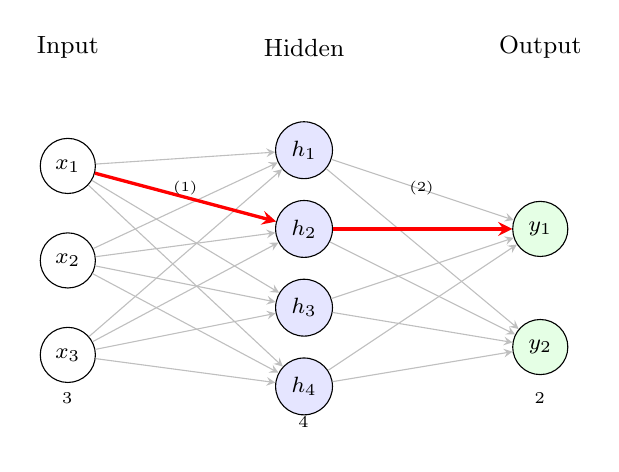
\begin{tikzpicture}[
    neuron/.style={circle, draw, minimum size=0.7cm, font=\footnotesize},
    arrow/.style={->, >=stealth},
    layer/.style={font=\small}
]

% Input layer
\foreach \i in {1,2,3} {
    \node[neuron] (x\i) at (0, -\i*1.2) {$x_{\i}$};
}
% Layer labels at fixed coordinates
\node[layer] at (0, 0.3) {Input};
\node[font=\footnotesize] at (0, -4.2) {$\R^3$};

% Hidden layer
\foreach \i in {1,2,3,4} {
    \node[neuron, fill=blue!10] (h\i) at (3, -\i*1) {$h_{\i}$};
}
\node[layer] at (3, 0.3) {Hidden};
\node[font=\footnotesize] at (3, -4.5) {$\R^4$};

% Output layer
\foreach \i in {1,2} {
    \node[neuron, fill=green!10] (y\i) at (6, -\i*1.5-0.5) {$y_{\i}$};
}
\node[layer] at (6, 0.3) {Output};
\node[font=\footnotesize] at (6, -4.2) {$\R^2$};

% Connections input to hidden (fully connected)
\foreach \i in {1,2,3} {
    \foreach \j in {1,2,3,4} {
        \draw[arrow, gray!50] (x\i) -- (h\j);
    }
}

% Connections hidden to output (fully connected)
\foreach \i in {1,2,3,4} {
    \foreach \j in {1,2} {
        \draw[arrow, gray!50] (h\i) -- (y\j);
    }
}

% Highlight one path
\draw[arrow, red, very thick] (x1) -- (h2);
\draw[arrow, red, very thick] (h2) -- (y1);

% Weight labels at fixed coordinates
\node[font=\tiny] at (1.5, -1.5) {$\mW^{(1)}$};
\node[font=\tiny] at (4.5, -1.5) {$\mW^{(2)}$};

\end{tikzpicture}
\caption{Multi-layer perceptron (MLP) computational graph showing fully-connected layers. Each neuron in the hidden layer receives input from \textbf{all} neurons in the input layer (12 connections total), and each output neuron receives input from all hidden neurons (8 connections). The red path highlights one example: $x_1 \to h_2 \to y_1$. This dense connectivity enables MLPs to learn complex non-linear functions.}
\label{fig:mlp_architecture}
\end{figure}

\begin{example}[3-Layer MLP for MNIST]
\label{ex:mnist_mlp}
Architecture for MNIST digit classification:
\begin{itemize}
    \item Input: $\vx \in \R^{784}$ (flattened $28 \times 28$ image)
    \item Hidden 1: $\vh^{(1)} \in \R^{256}$ with ReLU
    \item Hidden 2: $\vh^{(2)} \in \R^{128}$ with ReLU
    \item Output: $\vz^{(3)} \in \R^{10}$ with softmax
\end{itemize}

Parameter count: $200{,}960 + 32{,}896 + 1{,}290 = 235{,}146$ parameters.
\end{example}

\subsection{Why Depth Matters}

Without nonlinear activations, multiple layers collapse to single linear transformation. With nonlinearities, deep networks learn complex functions efficiently.

\section{Memory and Computation Analysis}
\label{sec:memory_computation}

For a single fully-connected layer computing $\vy = \mW\vx + \vb$ where $\mW \in \R^{m \times n}$, the forward pass requires approximately $2mn$ FLOPs and the backward pass requires approximately $4mn$ FLOPs (computing gradients with respect to inputs, weights, and biases). This gives a useful rule of thumb: one training step requires approximately $6\times$ as many FLOPs as the model has parameters---$2\times$ for the forward pass and $4\times$ for the backward pass. This ratio holds for fully-connected layers but varies with architecture; convolutional layers have much higher FLOPs per parameter due to weight sharing, while embedding layers have zero FLOPs (table lookups only).

During training, intermediate activations must be stored for the backward pass, and these often consume more memory than the model parameters. Activation memory scales linearly with batch size while parameter memory remains constant, so large batch sizes eventually become memory-limited. For transformer models, attention score matrices of size $B \times h \times n \times n$ dominate activation memory due to their $O(n^2)$ scaling with sequence length, dwarfing the $O(n)$ scaling of feed-forward activations.

Transformer feed-forward networks use a standard two-layer architecture with $4\times$ expansion: projecting from model dimension $d$ to $4d$ with a GELU activation, then back to $d$. For BERT-base ($d = 768$, expansion to 3072), the feed-forward networks contain approximately 4.7M parameters per layer and 56.6M across 12 layers, accounting for $\sim$51\% of total parameters. They similarly account for $\sim$54\% of total FLOPs, making them the largest single component in terms of both parameters and computation.

\section{Activation Functions}
\label{sec:activations}

\begin{definition}[ReLU]
\label{def:relu}
\begin{equation}
\text{ReLU}(z) = \max(0, z)
\end{equation}
Derivative: $\text{ReLU}'(z) = \mathbb{1}[z > 0]$
\end{definition}

\begin{definition}[GELU]
\label{def:gelu}
Gaussian Error Linear Unit (default in transformers):
\begin{equation}
\text{GELU}(z) = z \cdot \Phi(z)
\end{equation}
where $\Phi$ is standard normal CDF. Approximation:
\begin{equation}
\text{GELU}(z) \approx 0.5z \left(1 + \tanh\left[\sqrt{\frac{2}{\pi}}(z + 0.044715z^3)\right]\right)
\end{equation}
\end{definition}

\begin{keypoint}
Transformer models use GELU (BERT, GPT) or variants like Swish for feed-forward networks.
\end{keypoint}

\subsection{Computational Cost of Activation Functions}

GELU is 4$\times$ more expensive than ReLU in arithmetic operations, but in practice adds only 1--2\% to total training time because both operations are memory-bandwidth-bound on modern GPUs. Modern frameworks provide fused linear-activation kernels that eliminate intermediate memory traffic, providing 1.3--1.5$\times$ speedup for combined operations.

\subsection{Why GELU is Preferred in Transformers}

Despite its higher computational cost, GELU has become the standard activation function for transformer models, used in BERT, GPT-2, GPT-3, T5, and most modern language models. This preference is driven by empirical performance rather than computational efficiency: models trained with GELU consistently achieve better final accuracy than those trained with ReLU, particularly on language understanding tasks.

The theoretical motivation for GELU is that it provides a smoother approximation to the ReLU function, with non-zero gradients for negative inputs. While ReLU has gradient zero for all $z < 0$, GELU has small but non-zero gradients in this region, allowing the network to recover from neurons that have been pushed into the negative regime. This property is particularly valuable in deep networks where gradient flow through many layers can be fragile. For a 24-layer BERT-large model, the probability that a gradient signal survives through all layers is significantly higher with GELU than with ReLU, as GELU never completely blocks gradient flow.

Empirically, BERT-base trained with GELU achieves 84.6\% accuracy on the MNLI natural language inference task, compared to 83.9\% with ReLU—a 0.7 percentage point improvement that is statistically significant and practically meaningful. For GPT-2, the perplexity on the WebText validation set is 18.3 with GELU compared to 19.1 with ReLU, indicating better language modeling performance. These improvements justify the 1-2\% computational overhead of GELU, as the improved model quality translates to better downstream task performance and potentially reduced training time to reach a target accuracy.

The success of GELU has inspired variants like Swish and Mish that share the property of smooth, non-zero gradients everywhere. Swish, defined as $\text{Swish}(z) = z \cdot \sigma(z)$, has similar performance to GELU on most tasks and is used in some efficient transformer architectures like EfficientNet. Mish, defined as $\text{Mish}(z) = z \cdot \tanh(\text{softplus}(z))$, provides slightly better performance than GELU on some vision tasks but has higher computational cost. The landscape of activation functions continues to evolve, but GELU remains the standard for language models due to its strong empirical performance and reasonable computational cost.

\section{Universal Approximation Theorem}
\label{sec:universal_approximation}

\begin{theorem}[Universal Approximation]
\label{thm:universal_approximation}
A single-hidden-layer neural network with nonlinear activation can approximate any continuous function on compact domain to arbitrary precision, given sufficient hidden units.
\end{theorem}

Caveat: The theorem says nothing about how many units needed, how to find weights, or generalization. Deep networks often more efficient than wide networks.

\section{Weight Initialization}
\label{sec:weight_initialization}

\begin{definition}[Xavier Initialization]
\label{def:xavier_init}
For layer with $n_{\text{in}}$ inputs and $n_{\text{out}}$ outputs:
\begin{equation}
w_{ij} \sim \mathcal{N}\left(0, \frac{2}{n_{\text{in}} + n_{\text{out}}}\right)
\end{equation}
Best for tanh and sigmoid activations.
\end{definition}

\begin{definition}[He Initialization]
\label{def:he_init}
For ReLU networks:
\begin{equation}
w_{ij} \sim \mathcal{N}\left(0, \frac{2}{n_{\text{in}}}\right)
\end{equation}
Accounts for ReLU zeroing half the activations.
\end{definition}

\subsection{Variance Preservation Through Layers}

Proper weight initialization ensures that activations and gradients maintain reasonable magnitudes as they propagate through deep networks. Consider a linear layer $\vy = \mW\vx$ where $\vx \in \R^{n_{\text{in}}}$ has zero mean and unit variance, and weights $w_{ij}$ are independent with zero mean and variance $\sigma_w^2$. The variance of each output element is:
\begin{equation}
\text{Var}(y_i) = \text{Var}\left(\sum_{j=1}^{n_{\text{in}}} w_{ij} x_j\right) = \sum_{j=1}^{n_{\text{in}}} \text{Var}(w_{ij}) \text{Var}(x_j) = n_{\text{in}} \sigma_w^2
\end{equation}

To preserve variance ($\text{Var}(y_i) = 1$), we need $\sigma_w^2 = 1/n_{\text{in}}$. Xavier initialization uses $\sigma_w^2 = 2/(n_{\text{in}} + n_{\text{out}})$ to balance forward and backward pass variance preservation. For ReLU activations, which zero out half the activations on average, He initialization compensates by using $\sigma_w^2 = 2/n_{\text{in}}$, doubling the variance to maintain signal strength after the nonlinearity.

Without proper initialization, deep networks fail to train: with variance too large ($\sigma_w^2 = 1$), activations explode exponentially through layers; with variance too small ($\sigma_w^2 = 0.01$), they vanish to zero. For transformer models with GELU activations, He initialization or slight variants work well and are used universally in BERT, GPT, T5, and other modern architectures.

\section{Regularization}
\label{sec:regularization}

\subsection{L2 Regularization}

Add penalty to loss:
\begin{equation}
L_{\text{total}} = L_{\text{data}} + \frac{\lambda}{2} \sum_{\ell} \norm{\mW^{(\ell)}}_F^2
\end{equation}

L2 regularization, also known as weight decay, penalizes large parameter values to prevent overfitting. The regularization term adds the squared Frobenius norm of all weight matrices to the loss function, encouraging the optimizer to keep weights small. The hyperparameter $\lambda$ controls the strength of regularization: larger $\lambda$ produces smaller weights and stronger regularization.

The computational cost of L2 regularization is modest. Computing the squared norm $\norm{\mW}_F^2 = \sum_{ij} w_{ij}^2$ requires one multiplication and one addition per parameter, totaling $2P$ operations for a model with $P$ parameters. For BERT-base with 110 million parameters, this requires 220 million operations, or 0.22 GFLOPs. Compared to the 96 GFLOPs required for a forward pass, the regularization computation adds only 0.23\% overhead. On an NVIDIA A100 GPU, computing the regularization term takes approximately 0.7 microseconds, which is negligible compared to the 50 milliseconds for a full forward-backward pass.

The gradient of the L2 regularization term is even simpler: $\nabla_{\mW} \left(\frac{\lambda}{2} \norm{\mW}_F^2\right) = \lambda \mW$. This adds a term proportional to the current weights to the gradient, which can be implemented as a simple scaling operation during the optimizer step. Most optimizers, including PyTorch's Adam and SGD, support weight decay as a built-in parameter that applies this scaling automatically without requiring explicit computation of the regularization term. This makes L2 regularization essentially free from a computational perspective.

The memory overhead of L2 regularization is zero, as it requires no additional storage beyond the parameters themselves. The regularization term is computed on-the-fly during the backward pass and does not need to be stored. This makes L2 regularization an attractive regularization technique for large models where memory is at a premium.

\subsection{Dropout}

\begin{definition}[Dropout]
\label{def:dropout}
During training, randomly set activations to zero with probability p. During inference, scale by $(1-p)$.
\end{definition}

Dropout is a powerful regularization technique that randomly drops (sets to zero) a fraction of activations during training. This prevents the network from relying too heavily on any single neuron and encourages learning robust features. The dropout probability $p$ is typically 0.1 to 0.5, with higher values providing stronger regularization at the cost of slower convergence.

\subsection{Dropout in Practice}

Dropout adds approximately 4--5\% overhead to training time for BERT-base, primarily from random number generation and memory traffic for the binary mask. Transformer models apply dropout at multiple points: after attention weights (attention dropout), after sublayer outputs (residual dropout), and on input embeddings. BERT uses $p=0.1$ at all locations; GPT-3 uses only residual dropout.

\section{Exercises}

\begin{exercise}
Design 3-layer MLP for binary classification of 100-dimensional inputs. Specify layer dimensions, activations, and parameter count.
\end{exercise}

\begin{exercise}
Compute forward pass through 2-layer network with given weights and ReLU activation.
\end{exercise}

\begin{exercise}
For layer with 512 inputs and 256 outputs using ReLU: (1) What is He initialization variance? (2) Why different from Xavier? (3) What happens with zero initialization?
\end{exercise}

\begin{exercise}
Prove that without nonlinear activations, L-layer network equivalent to single layer.
\end{exercise}

\section{Solutions}

\begin{solution}[Exercise 1]
\textbf{3-layer MLP design for binary classification:}

\textbf{Architecture:}
\begin{itemize}
    \item Input layer: 100 dimensions
    \item Hidden layer 1: 100 $\to$ 64 with ReLU activation
    \item Hidden layer 2: 64 $\to$ 32 with ReLU activation
    \item Output layer: 32 $\to$ 1 with sigmoid activation
\end{itemize}

\textbf{Parameter count:}
\begin{itemize}
    \item Layer 1: $\mW^{(1)} \in \R^{64 \times 100}$ has $6{,}400$ weights, $\vb^{(1)} \in \R^{64}$ has $64$ biases
    \item Layer 2: $\mW^{(2)} \in \R^{32 \times 64}$ has $2{,}048$ weights, $\vb^{(2)} \in \R^{32}$ has $32$ biases
    \item Layer 3: $\mW^{(3)} \in \R^{1 \times 32}$ has $32$ weights, $b^{(3)} \in \R$ has $1$ bias
    \item Total: $6{,}400 + 64 + 2{,}048 + 32 + 32 + 1 = 8{,}577$ parameters
\end{itemize}

\textbf{Forward pass equations:}
\begin{align}
\vh^{(1)} &= \text{ReLU}(\mW^{(1)}\vx + \vb^{(1)}) \\
\vh^{(2)} &= \text{ReLU}(\mW^{(2)}\vh^{(1)} + \vb^{(2)}) \\
\hat{y} &= \sigma(\mW^{(3)}\vh^{(2)} + b^{(3)})
\end{align}

where $\sigma(z) = \frac{1}{1 + e^{-z}}$ is the sigmoid function.
\end{solution}

\begin{solution}[Exercise 2]
\textbf{Forward pass computation:}

Given weights:
\begin{equation}
\mW^{(1)} = \begin{bmatrix} 0.5 & -0.3 \\ 0.2 & 0.6 \end{bmatrix}, \quad \vb^{(1)} = \begin{bmatrix} 0.1 \\ -0.2 \end{bmatrix}, \quad \mW^{(2)} = \begin{bmatrix} 1.0 & -0.5 \end{bmatrix}, \quad b^{(2)} = 0.3
\end{equation}

Input: $\vx = \begin{bmatrix} 2.0 \\ 1.0 \end{bmatrix}$

\textbf{Layer 1:}
\begin{align}
\vz^{(1)} &= \mW^{(1)}\vx + \vb^{(1)} = \begin{bmatrix} 0.5(2.0) - 0.3(1.0) \\ 0.2(2.0) + 0.6(1.0) \end{bmatrix} + \begin{bmatrix} 0.1 \\ -0.2 \end{bmatrix} = \begin{bmatrix} 0.8 \\ 0.8 \end{bmatrix} \\
\vh^{(1)} &= \text{ReLU}(\vz^{(1)}) = \begin{bmatrix} 0.8 \\ 0.8 \end{bmatrix}
\end{align}

\textbf{Layer 2:}
\begin{align}
z^{(2)} &= \mW^{(2)}\vh^{(1)} + b^{(2)} = 1.0(0.8) - 0.5(0.8) + 0.3 = 0.7 \\
\hat{y} &= z^{(2)} = 0.7 \quad \text{(no activation for regression)}
\end{align}

Final output: $\hat{y} = 0.7$
\end{solution}

\begin{solution}[Exercise 3]
For layer with 512 inputs and 256 outputs using ReLU:

\textbf{(1) He initialization variance:}
\begin{equation}
\text{Var}(w_{ij}) = \frac{2}{n_{\text{in}}} = \frac{2}{512} = 0.00391
\end{equation}

Standard deviation: $\sigma = \sqrt{0.00391} \approx 0.0625$

\textbf{(2) Why different from Xavier:}
\begin{itemize}
    \item Xavier initialization: $\text{Var}(w) = \frac{1}{n_{\text{in}}}$ (for tanh/sigmoid)
    \item He initialization: $\text{Var}(w) = \frac{2}{n_{\text{in}}}$ (for ReLU)
    \item ReLU zeros out half the activations, reducing variance by factor of 2
    \item He initialization compensates by doubling the initial variance
    \item This maintains signal variance through deep networks with ReLU
\end{itemize}

\textbf{(3) Zero initialization problem:}
If all weights are initialized to zero:
\begin{itemize}
    \item All neurons in a layer compute identical outputs
    \item All gradients are identical (symmetry)
    \item Neurons never differentiate during training
    \item Network effectively has only one neuron per layer
    \item Learning fails completely
\end{itemize}

Random initialization breaks symmetry, allowing neurons to learn different features.
\end{solution}

\begin{solution}[Exercise 4]
\textbf{Proof that L-layer linear network equals single layer:}

Consider an $L$-layer network without nonlinear activations:
\begin{align}
\vh^{(1)} &= \mW^{(1)}\vx + \vb^{(1)} \\
\vh^{(2)} &= \mW^{(2)}\vh^{(1)} + \vb^{(2)} \\
&\vdots \\
\vh^{(L)} &= \mW^{(L)}\vh^{(L-1)} + \vb^{(L)}
\end{align}

Substituting recursively:
\begin{align}
\vh^{(2)} &= \mW^{(2)}(\mW^{(1)}\vx + \vb^{(1)}) + \vb^{(2)} \\
&= \mW^{(2)}\mW^{(1)}\vx + \mW^{(2)}\vb^{(1)} + \vb^{(2)}
\end{align}

Continuing to layer $L$:
\begin{align}
\vh^{(L)} &= \mW^{(L)}\mW^{(L-1)}\cdots\mW^{(1)}\vx + \text{(bias terms)} \\
&= \mW_{\text{eff}}\vx + \vb_{\text{eff}}
\end{align}

where:
\begin{align}
\mW_{\text{eff}} &= \mW^{(L)}\mW^{(L-1)}\cdots\mW^{(1)} \\
\vb_{\text{eff}} &= \sum_{i=1}^{L} \left(\prod_{j=i+1}^{L} \mW^{(j)}\right) \vb^{(i)}
\end{align}

This is equivalent to a single linear layer with weights $\mW_{\text{eff}}$ and bias $\vb_{\text{eff}}$. Therefore, without nonlinear activations, depth provides no additional representational power—the network can only learn linear functions regardless of depth.
\end{solution}

